\documentclass{article}
\usepackage{subfiles}
\usepackage{graphicx}
\usepackage{fancyhdr}
\usepackage{tabularx}
\usepackage{listings}
\usepackage{float}
\usepackage[french]{babel}

\pagestyle{fancy}
\fancyhf{} % Efface les en-têtes et pieds de page par défaut
\fancyfoot[R]{\thepage} % Aligne le numéro de page à droite en bas
\renewcommand{\headrulewidth}{0pt} % Supprime la ligne en haut de page
\renewcommand{\footrulewidth}{0pt} % Supprime la ligne en bas de page

\begin{document}

\title{Document de conception \\ SAE S4.Deploi.01}
\author{Tristan Petit, Nils Hubert, Toni Rey,\\ 
 Majd El Sebeiti , Vianney Miquel}
\date{\today}
\maketitle

\begin{center}
    \vspace{1cm} % Espace entre la date et l'image
    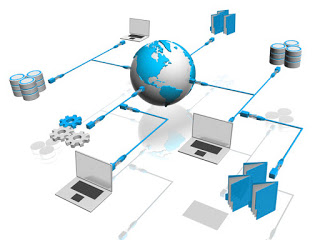
\includegraphics{Images/Logo-project.jpeg} % Ajuste le chemin et la taille
\end{center}

\newpage
\pagenumbering{gobble} % Désactive la numérotation de page pour la table des matières
\renewcommand{\contentsname}{Table des matières} % Titre personnalisé de la table des matières

\tableofcontents 

\newpage


\pagenumbering{arabic} % Reprend la numérotation des pages

%==================================%
%  INCLUSION DU MODULE POUR INTRO  %
%==================================%

\section{Introduction}

\subfile{Introduction/introduction.tex}

\newpage

%==================================%
%  INCLUSION DU MODULE POUR Architeceure  %
%==================================%

\section{Rappel et évolution sur l'architecture}

\subfile{Architecture/architecture.tex}

\newpage

\section{Scripte crée }

\subfile{scripte/scipte.tex}

\newpage

\section{Ressources utilisées}

Pour notre SAE, nous avons réuni les machines dans un cluster pour interconnecter nos hyperviseurs et mutualiser les ressources qui sont réparties à travers nos hyperviseurs.

\begin{figure}[h]
    \centering
    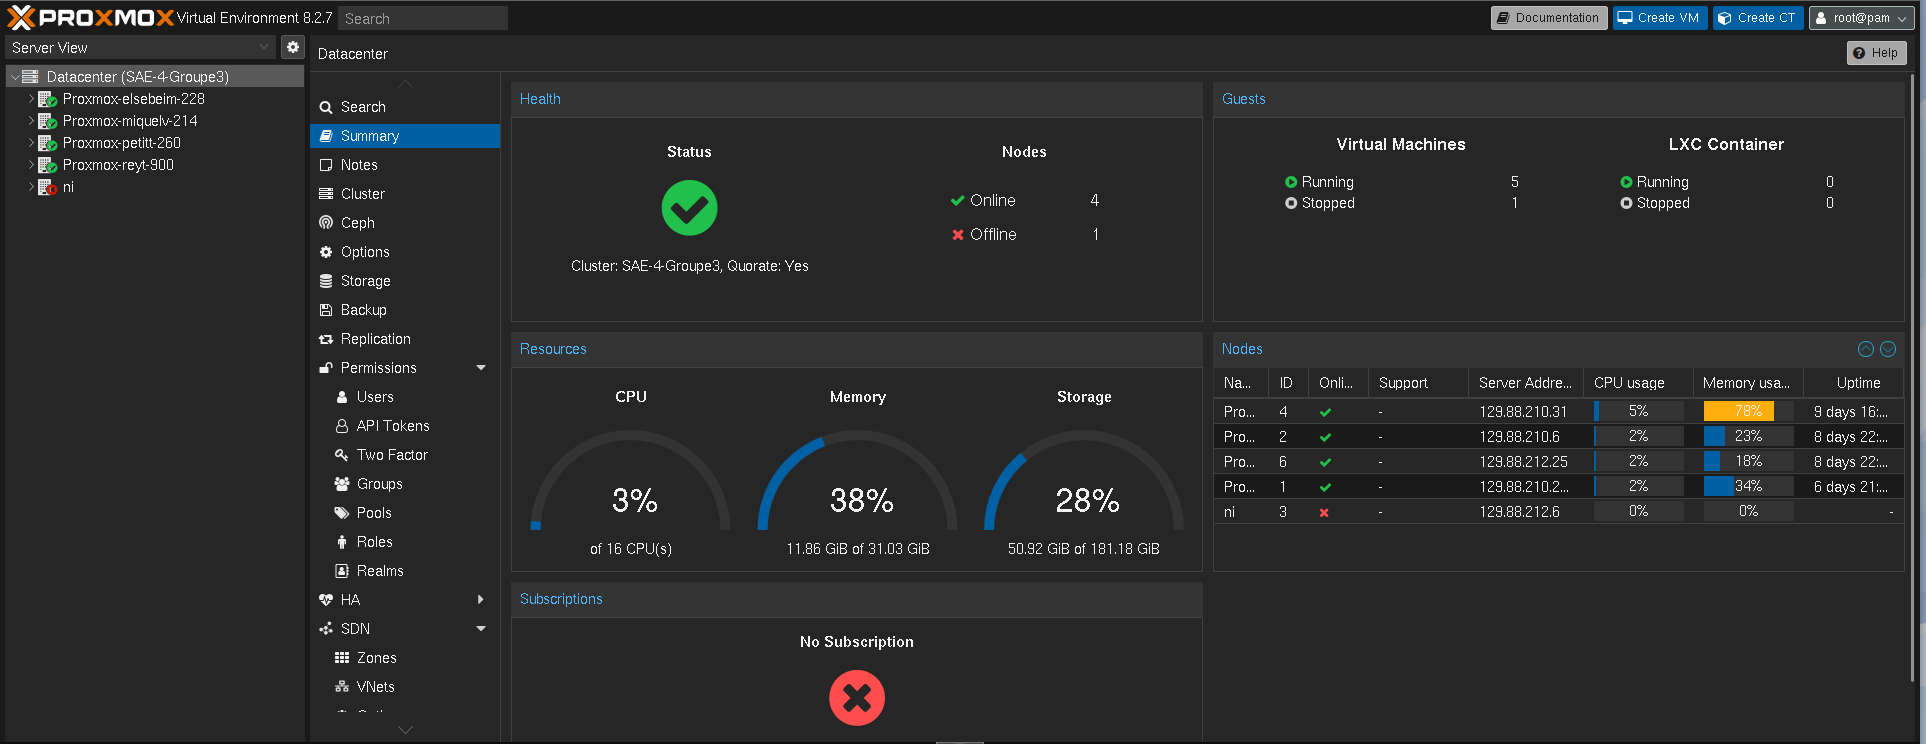
\includegraphics[width=1\textwidth]{Images/Ressource.png}
    \caption{Ressource utilisée pour la SAE sous proxmox}
    \label{fig:solution1}
\end{figure}

L'avantage de cette configuration par rapport à celle présente sur ASSR, c'est que nous n'avons pas de machines virtuelles imbriquées, ce qui permet d'améliorer de manière significative les performances. \\
Le CPU est la ressource qui pose le moins de problème dans notre cas, il en est tout autre pour la RAM. Celle-ci devra être gérée de manière équitable entre les hyperviseurs pour éviter une surcharge. 
Le stockage ne devrait pas poser de problème majeur, mais pourrait le devenir si nous étions dans l'obligation d'ajouter de nouvelles machines.

\newpage

\section{Documentation Technique}

\subfile{DocTechnique/DNS/DNS.tex}
%\subfile{DocTechnique/routeurs/routeurs.tex}

\end{document}
